\chapter{Goby MOOS Modules}\label{chap:MOOS}
\MakeShortVerb{\!} % makes !foo! == !foo!

The acoustic communications portion of Goby was developed originally for the MOOS autonomy architecture. Thus, the relevant MOOS modules !pAcommsHandler! and others are still maintained (in goby/src/moos) for the use of the !MOOS-IvP! community. !MOOS-IvP! is explained in \cite{moos-ivp-jfr} and is available at \url{http://moos-ivp.org}. The usage of these modules is documented here. See \url{http://gobysoft.com/doc/#install} for how to install Goby.

The beginning of this appendix motivates the design, followed by a detailed user manual for the individual MOOS processes.

\section{Unified Command and Control for Subsea Autonomous Sensing Networks}

The process of undersea observation, mapping, and monitoring is experiencing a dramatic
paradigm shift away from platform-centric, human-controlled sensing,
processing and interpretation. Rather, distributed sensing
using networks of autonomous platforms is becoming the preferred technique.
An optimal platform suite is often highly heterogeneous with large differences in mobility,
maneuverability, sensing capability, and communication connectivity.  The
sensor systems have different constraints on platform mobility and
communication capacity, and some network operations require highly
coordinated maneuvering of heterogeneous platforms. Unified Command and Control \cite{unified_c2} is a new command and control paradigm inherently suited for such heterogeneous networks. Implemented using
!MOOS-IvP!, Unified C2 provides the fully integrated sensing,
modeling and control that allows each platform, on its own or in
collaboration with partners of opportunity, to autonomously detect,
classify, localize and track (DCLT) an episodic, natural or human-created event, and
subsequently report back to the operators.

A robust undersea communication infrastructure is crucial to the
operation of such networks. In contrast to air and land-based
equivalents, the extremely limited bandwidth, latency and
intermittency of underwater acoustic communication imposes severe
requirements to the selectivity of message handling. Thus, contact and
track reports for high-priority event, such as a detected chemical
plume from a deep ocean vent,  which may indicate an imminent volcanic
eruption, must be transmitted to the system operators without delay. On the
other hand, reports concerning less important events and platform status 
reports may be delayed without significant effects.
Previous message handling systems for underwater communications have only a
rigid, hard-coded queuing infrastructure, and do not support such
advanced priority-based selectivity, hampering the type and
amount of information that can be passed between cooperating nodes in
the network. This severely limits the level of autonomy that can be
supported on the network nodes.

\begin{figure}[tp]
  \centering 
  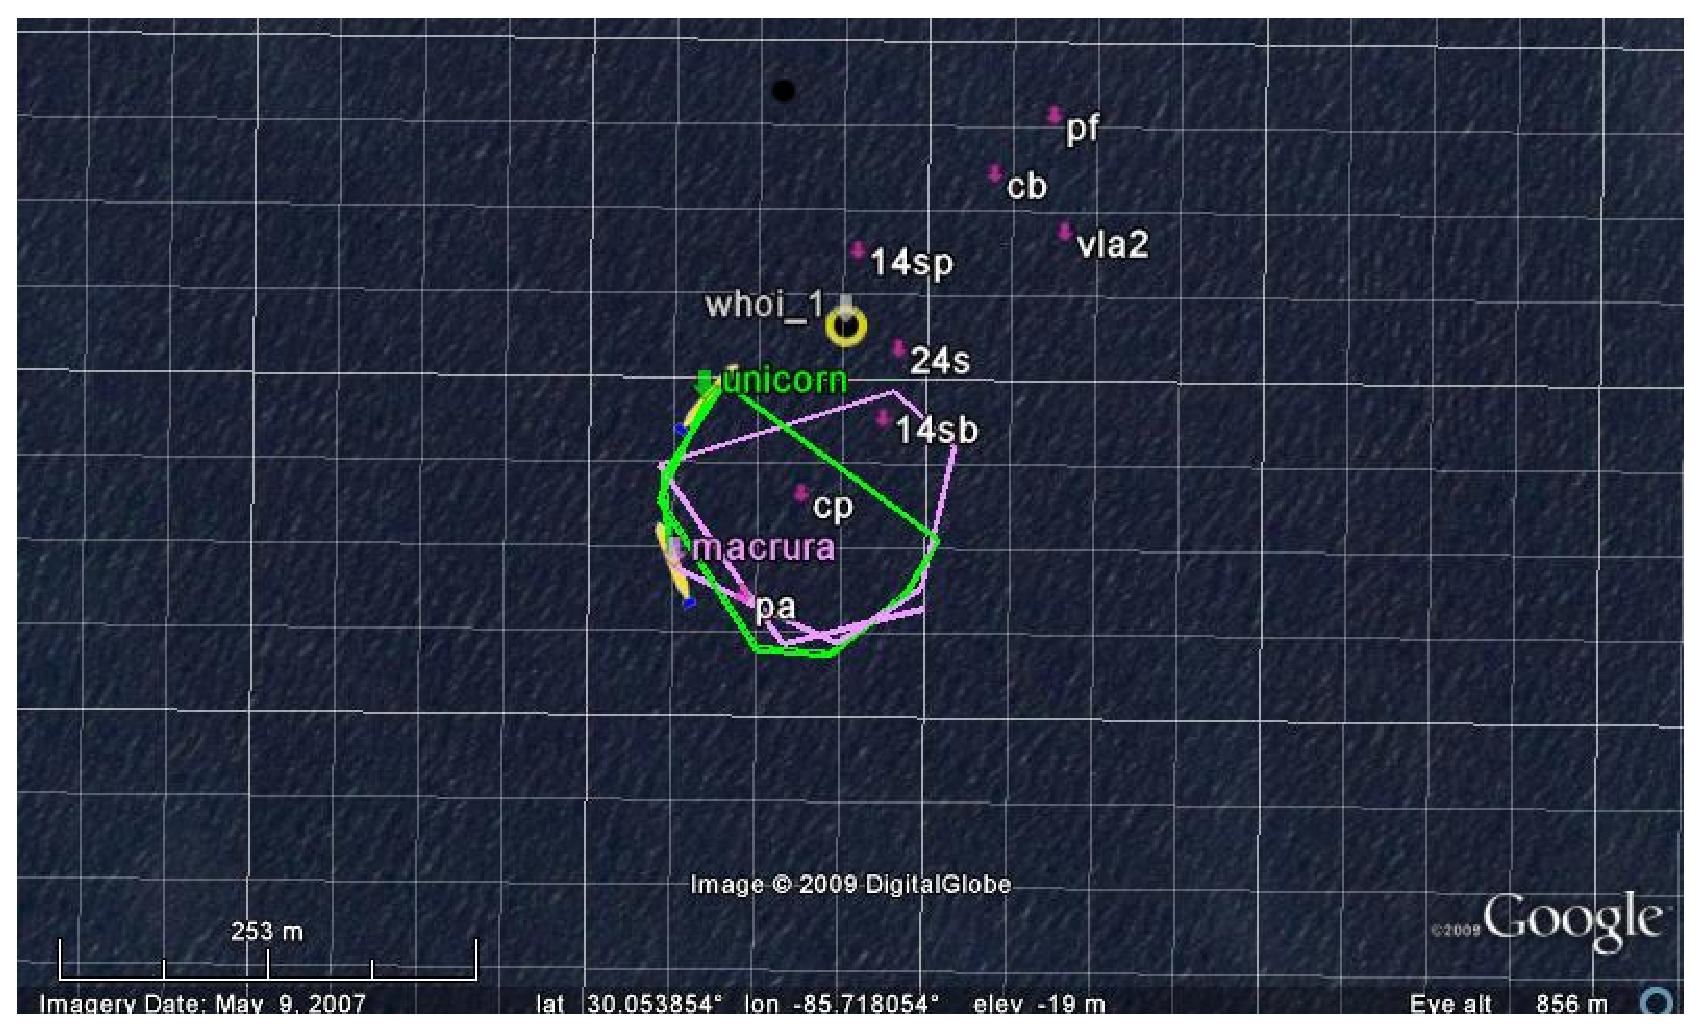
\includegraphics[width=0.75\textwidth]{bistatic3.eps}
\caption{ Collaborative autonomy demonstrated in SWAMSI09 using MIT
  LAMSS communication stack. The two BF21 AUVs Unicorn and Macrura
  perform synchronized swimming maintaining a constant bistatic angle
  of $60^{\circ}$ relative to a proud cylindrical target
  (cp). \label{bistatic3}}
\end{figure}

In response to this problem, a new !MOOS-IvP! communication software stack was developed at
the MIT \gls{lamss} \cite{lamss}, in
support of autonomous sensing programs such as the ONR ASAP MURI,
GOATS, and SWAMSI. This new stack has enabled the operation of a communication
infrastructure which provides robust message handling for
collaborative autonomous sensing by heterogeneous, undersea autonomous
assets, as demonstrated in a handful of major recent field
experiments. As an example, Fig.~\ref{bistatic3} shows the
collaborative, multistatic MCM mission by the Unicorn and Macrura BF21
AUVs during SWAMSI09 in Panama City, FL. The two vehicles are circling
a proud cylinder (cp) at a distance of 80 m maintaining a constant
bistatic angle of 60 degrees. The collaboration was achieved fully
autonomously without any intervention by the operators, with each
vehicle adapting its speed based on its current position and the
position of the other vehicle extrapolated from the latest status,
contact or track report. Such collaborative maneuvers would not be
possible using traditional communication schemes, where navigation
packets must be rigidly interleaved with messages containg data and
command and control sequences. In contrast, the Dynamic Compact
Control Language (DCCL) used by the \gls{lamss} communication
stack allows for adequate navigation information to be packed with all
other required message content.

Being based on the established open source !goby-acomms! libraries of message handling software, the
open source architecture of this new MOOS communication stack (embodied primarily in the MOOS application !pAcommsHandler! lends
itself directly to a wide range of military and civilian
applications. It supports an arbitrary message suite and
content without requirement of modifying software. All message encoding and
decoding information is specified in a mission-unique configuration
file written in the standard XML format. Not only does this ensure
maximum flexibility in regard to message design, but it inherently
enables arbitrary levels of encryption for LPI/LPD communication
networks.

\section{Overview of the LAMSS Communication Stack}

\begin{figure}[tp]
  \centering 
  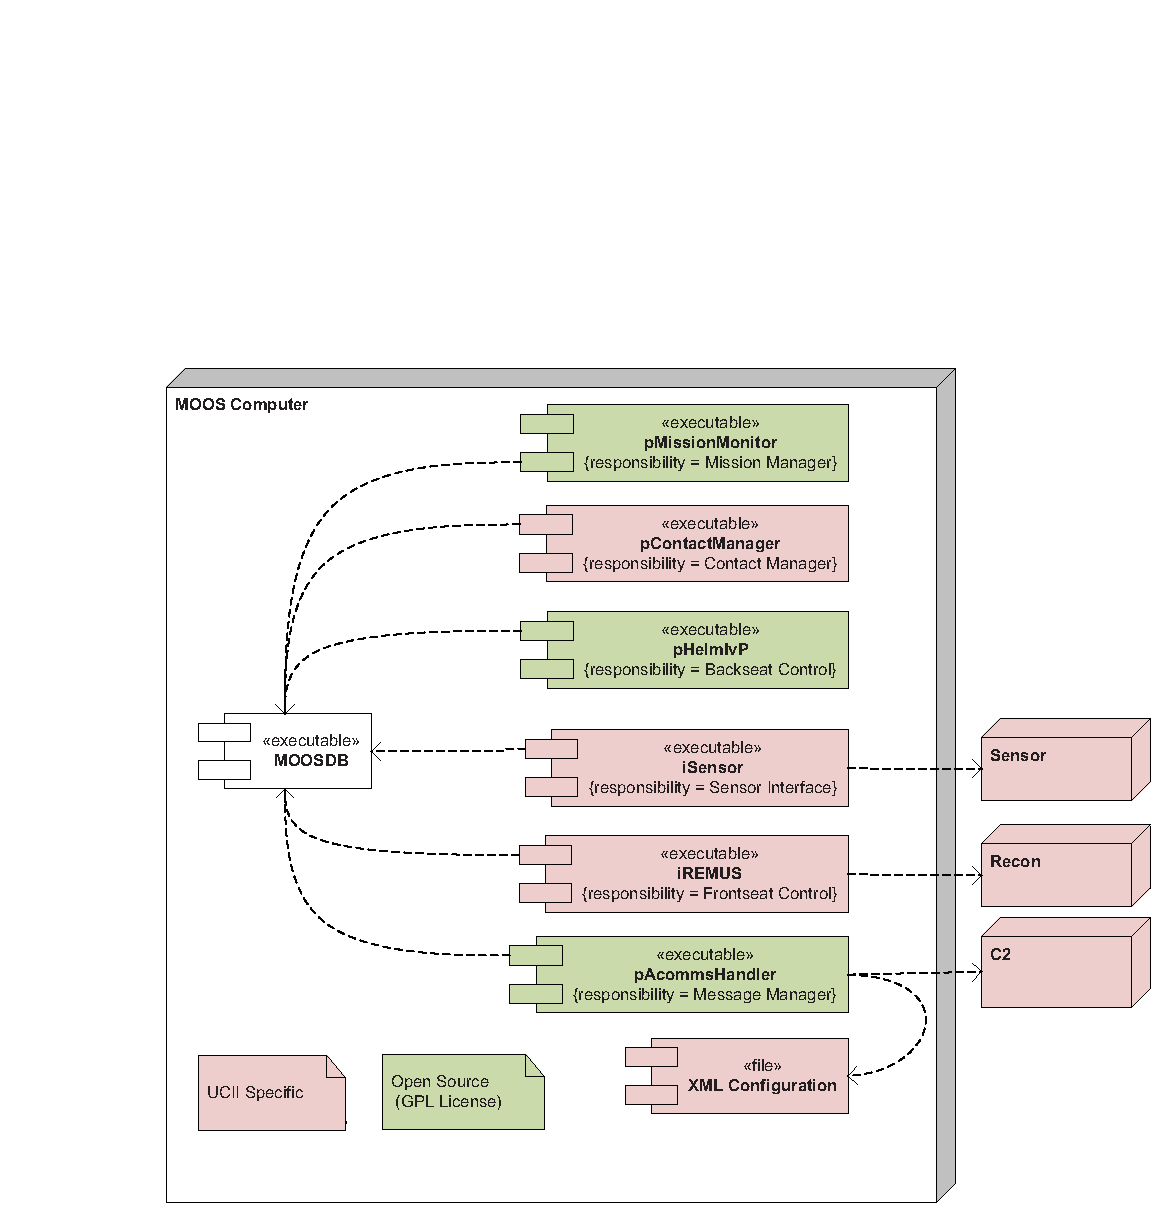
\includegraphics[width=\textwidth]{dclt_component.eps}
\caption{Incorporation of the open source LAMSS communication stack into
 a \texttt{MOOS-IvP} DCLT Autonomy System. The green boxes identify the
 open source modules, including the IvP Helm, the generic mission
 manager module, and the communication stack. The red modules are
 project specific, including the frontseat driver module, and the
 sensor modules. Also the message configuration specifying the message
 content and the coding, is project specific. \label{lamss_dclt}} 
\end{figure}

MIT \gls{lamss} \cite{lamss} has over the last decade focused its research on the
development of sensor-adaptive, collaborative, autonomous sensing
concepts for the capture of episodic undersea events, including the
mapping of coastal fronts, chemical plumes, and natural and man-made
underwater acoustic sources. All these applications involve the
Detection, Classification, Localization and Tracking (DCLT) of the
event. To exploit the benefits of having multiple platforms involved
in tracking the event, an underwater robust communication system is
obviously a requirement. On the other hand, the communication capacity
of such systems is many orders of magnitude below land- and air-based
equivalents, requiring a much higher level of data compression and
on-board processing and decision-making than is required in air-based
systems. Unified C2 \cite{unified_c2}, developed over the
last decade by \gls{lamss}, is an example of such an autonomy-driven
undersea sensing concept. Although this concept is based on the
philosophy that the system must be able to achieve its mission
objective even during periods with no or limited communication, there
is obviously still a need for occasional communication, e.g. for
reporting detected events of interest.

The new !MOOS-IvP! communication stack alleviates some of the problems and limitations of the
existing software stacks in this regard. These software stacks in general were designed to
sequentially transmit all messages generated by the autonomy system,
with only a rigid, hard-coded priority-based message queuing
infrastructure.

In undersea autonomous systems the priorities of information generated
by the on-board processing are highly dynamic, depending on the
tactical situation and the criticality of the generated
information. Thus, for example, a contact report for a target of
interest obviously must bypass queued contact reports for less
significant targets. Also, in high-clutter environments, the number of
contact reports may by far exceed the communication capacity and on-board
priority-based filtering is required.

\begin{figure}[htp]
\centering 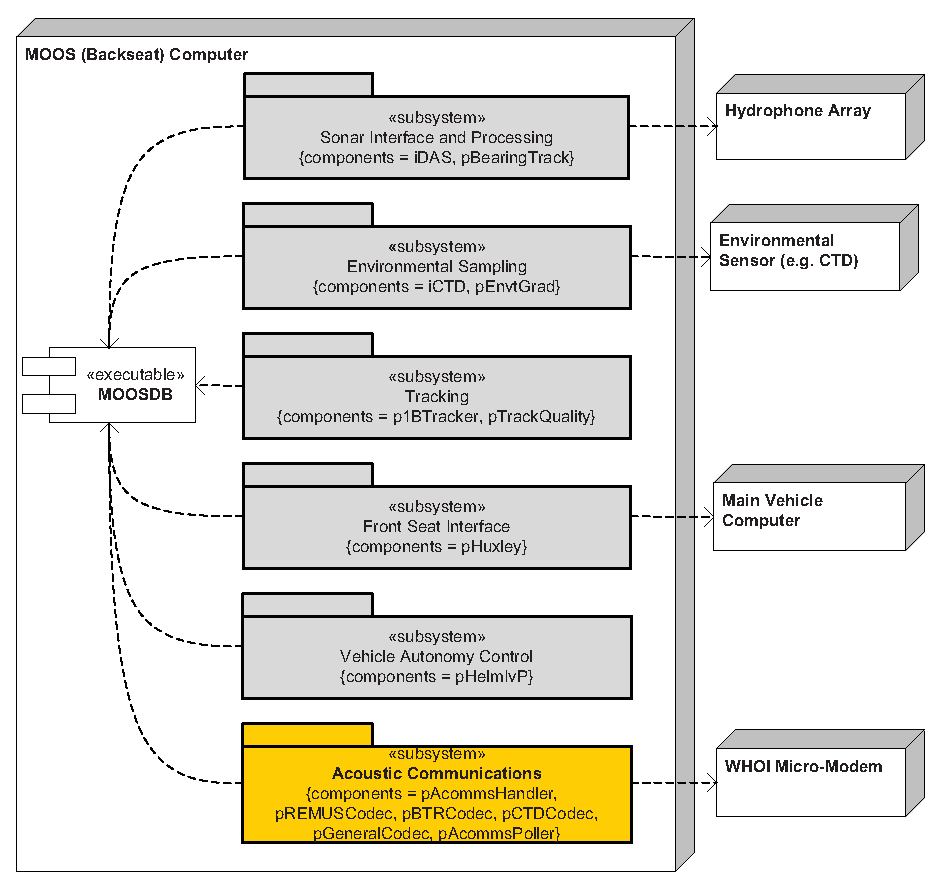
\includegraphics[width=\linewidth]{auv_community.eps}
\caption{\texttt{MOOS-IvP} community for MIT sonar AUVs, with the autonomous
  communication, command and control modules highlighted in
  gold. }
\label{fig:moos_comms}
\end{figure}

The incorporation of the MIT \gls{lamss} communication stack into a MOOS-IvP
DCLT Autonomy System is illustrated in Fig.~\ref{lamss_dclt}. The
green boxes identify the Open Source modules, including the helm !pHelmIvP!, the generic mission manager module !pMissionMonitor!,
and the communication stack. The red modules are project-specific,
including the frontseat driver module !iRemus!, the sensor
modules, and the contact manager process !pContactManager!. Also
the message configuration files specifying the message content and the
coding specifics, are project-specific and not hard-wired into the
communication stack.

Figure \ref{fig:moos_comms} shows the communications subsystem as part of the whole
MIT LAMSS AUV MOOS community.


 Figure \ref{acomms_sequence} shows the sequence of commands for a single operator command message sent using iCommander.
 
 
\begin{figure}[tp]
  \centering 
  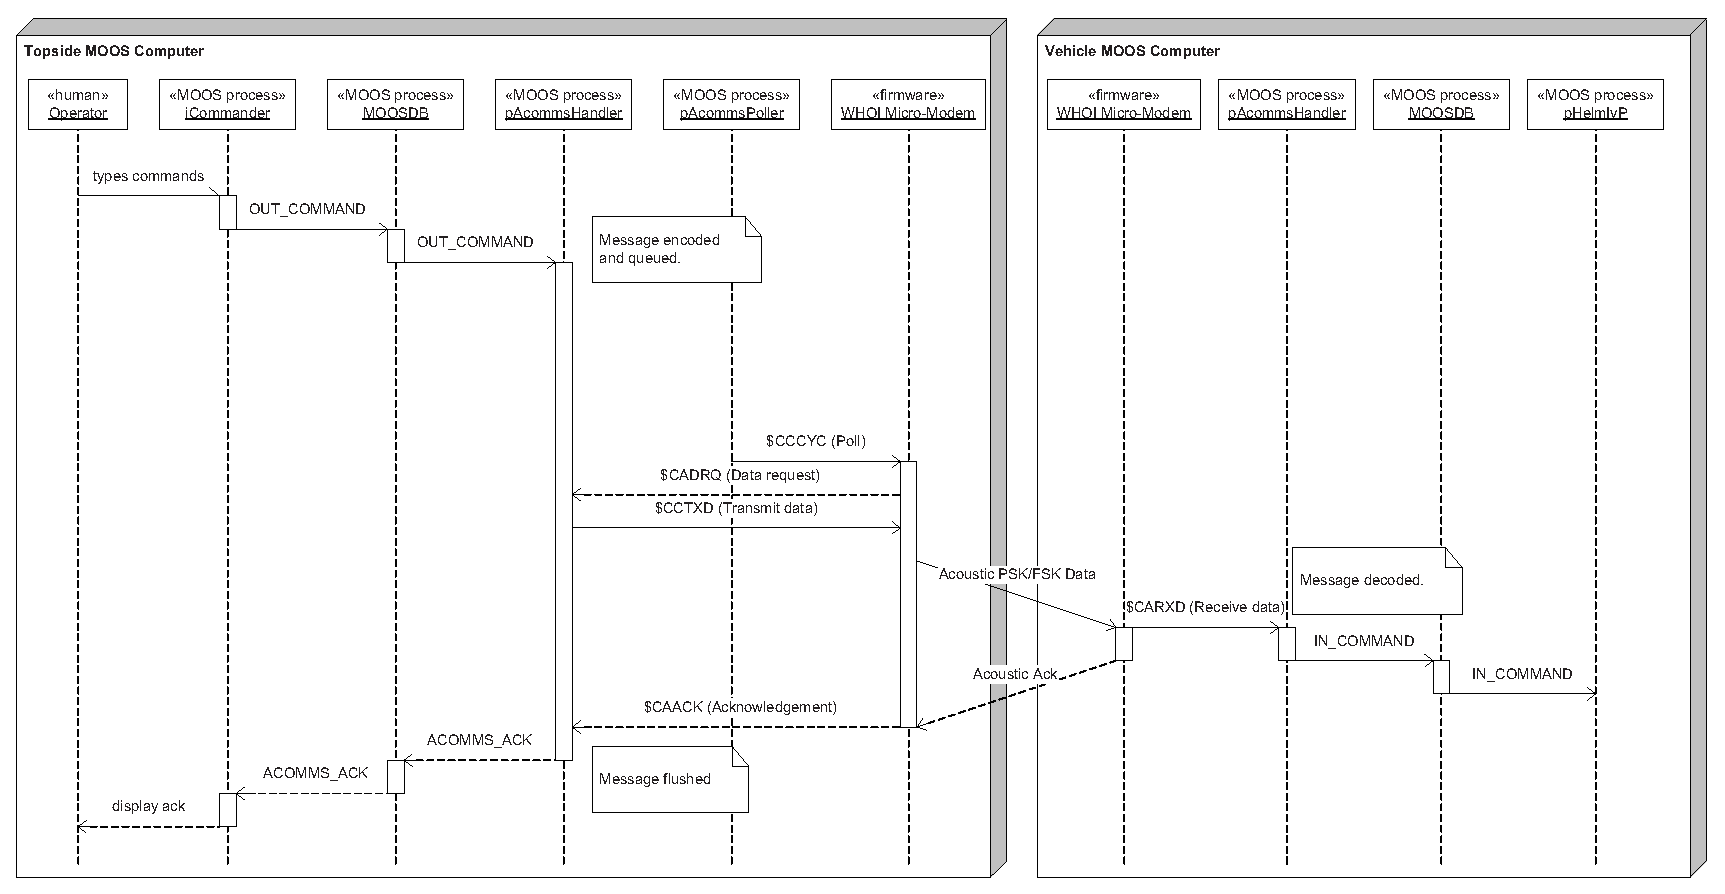
\includegraphics[width=1\textwidth]{acomms_sequence.eps}
\caption{UML Sequence diagram for sending a command to an AUV via the LAMSS Acoustic Communications Modules. \label{acomms_sequence}}
\end{figure}


The structure of the MIT LAMSS communication stack
is illustrated in Fig.~\ref{lamss_comms}.

\begin{figure}[tp]
  \centering 
  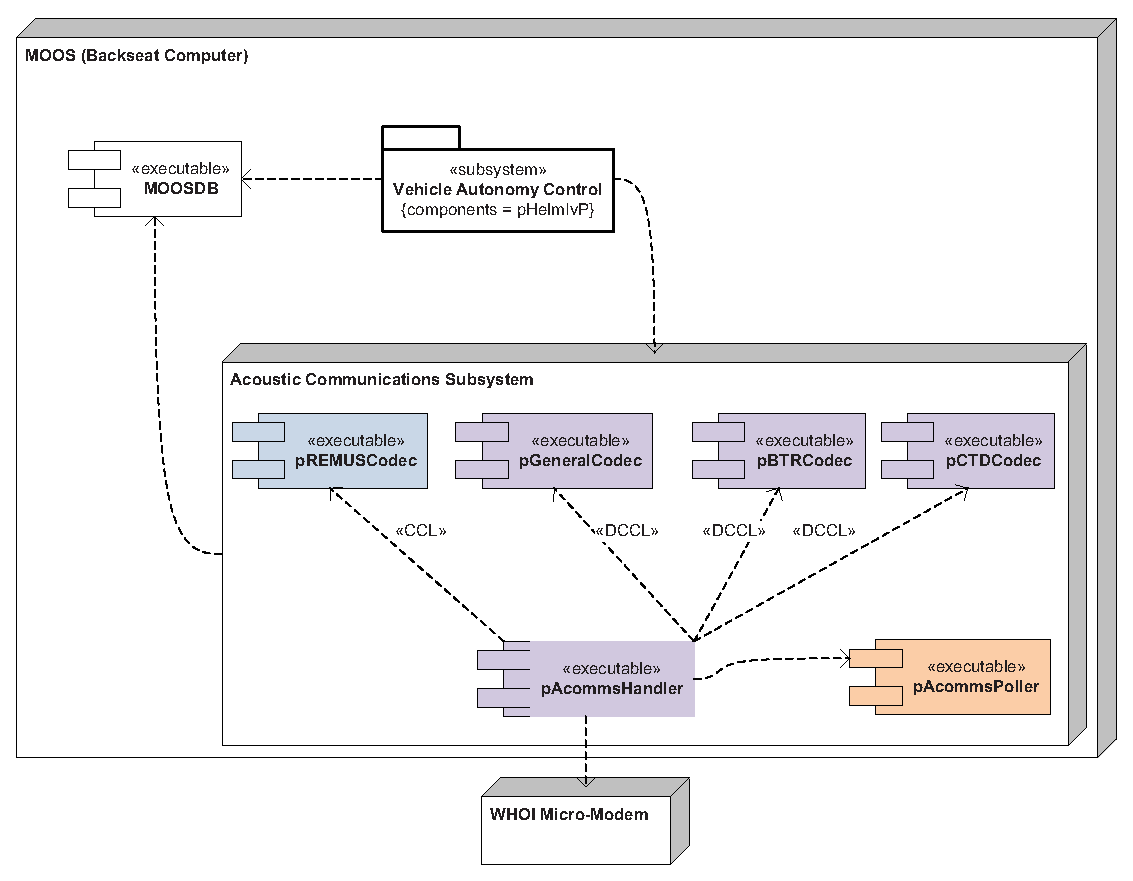
\includegraphics[width=\textwidth]{acomms_component.eps}
  \caption{UML Component Model of the MIT LAMSS communication stack. The principal
  message handler module is \texttt{pAcommsHandler}, which communicates
  directly with the modem using built-in drivers, and thus not
  dependent on third-party MOOS modem drivers. It also manages the
  message stream by a dynamic, priority-based queuing system. The
  message coding and decoding is performed by \texttt{pGeneralCodec} based on
  the rules set out in the configuration file, and dedicated DCCL
  codecs for transmitting various data streams.The stack also
  supports standard fixed Compact Control Language (CCL) messages such
  as the State message used by the Remus AUV, using dedicated codecs. Dashed line indicate dependencies between components. \label{lamss_comms}}
\end{figure}

\section{pAcommsHandler}
\label{sec:pacommshandler} 


\subsection{Problem}
Acoustic communications are highly limited in throughput. Thus, it is unreasonable to expect ``total throughput'' of all communications data. Furthermore, even if total throughput is achievable over time, certain messages have a lower tolerance for delay (e.g. vehicle status) than others (e.g. CTD sample data). Reference \url{http://acomms.whoi.edu/umodem/documentation.html} for more information on the WHOI Micro-Modem.

Also, in order to make the best use of this available bandwidth, messages need to be compacted to a minimal size before sending (effective encoding). To do this, pAcommsHandler provides an interface to the Dynamic Compact Control Language (DCCL\footnote{the name comes from the original CCL written by Roger Stokey for the REMUS AUVs, but with the ability to dynamically reconfigure messages based on mission need. DCCL is backwards compatible with a CCL network as it uses CCL message number 32}.) encoder/decoder. Furthermore, DCCL has powerful parsing abilities (``algorithms'') for both encoding and decoding, including the ability to perform certain geodesic conversions (e.g. latitude, longitude $\leftrightarrow$ UTM x,y) and lookups (e.g. \textit{modem\_id} $\leftrightarrow$ vehicle name) on data.

pAcommsHandler roughly performs the same functions of pFramer, pRouter, pAcommsPoller, and iMicroModem but
generalized to handle any number of message queues and extended to give more control over queue parameters. The DCCL encoding is much more flexible and more compact than the CCL encoding used by these older processes.

\subsection{Solution}
pAcommsHandler provides a(n):
\begin{enumerate}
\item Encoder/decoder unit (codec): encodes and decodes messages using DCCL (goby-acomms !dccl! library), which reduces the data required to be sent by:
\begin{itemize}
\item Predefined messages: the user must specify a message structure what specifies what fields the message contains and how large each field should be (in an intuitive fashion that DCCL turns into bits). Both the sender and receiver have preshared knowledge of the message structure. From this knowledge, no meta information about the message (beyond an identifier) needs to be sent, simply the data. 
\item Custom field sizes: message fields are defined with custom tolerances (ranges and precisions) that are tighter than those given by the IEEE standards for floating point and integer numbers. For example, if a field needs to hold an integer that will never range outside [0, 1000] that field in the message will only be 10 bits long (ceil($\log_2{1001}$)).
\end{itemize}
\item Priority Queuing System: maintains an arbitrary number of message queues (each tied to a different MOOS variable) for hexadecimal data strings. (goby-acomms !queue! library)
\begin{itemize} 
\item allows configuration of the queue priorities and dynamic growth of the priority over the time since the last sent message.
\item allows management of WHOI CCL message types as well as DCCL queuing. 
\end{itemize}
\item Modem Driver: handles all Micro-Modem serial communications. The driver (goby-acomms !modemdriver! library) can be used with other modems besides the WHOI Micro-Modem (see \url{http://gobysoft.com/doc/acomms__driver.html#acomms_writedriver} for information on writing a new driver). 
\item MAC Manager: provides medium access control in the form of a simple slotted time division-multiple access (TDMA) scheme or flexible centralized polling (goby-acomms !amac! library).
\end{enumerate}

\subsection{Limitations}
pAcommsHandler \textit{does not}:

\begin{itemize}
\item presently provide any multi-hop routing. The sender and receiver must be directly connected acoustically.
\item split user messages into packets. The user must provide data that are small enough to fit into the modem frame desired (32 - 256 bytes for the WHOI Micro-Modem).
\end{itemize} 

\subsection{Compilation}
pAcommsHandler depends on the Goby and MOOS libraries. See goby/DEPENDENCIES for help resolving the dependencies on your system.

\subsection{Parameters for the pAcommsHandler Configuration Block}\label{sec:pAcommsHandler:config}

\subsubsection{Example moos file}

You can always get a complete listing of MOOS file parameters with their syntax by running
\begin{verbatim}
> pAcommsHandler --example_config
\end{verbatim}
\resetbvlinenumber

This is a complete list of all the configuration values pAcommsHandler accepts. Most of the time you will need far fewer configuration options to use it.

\boxedverbatiminput{"@RELATIVE_CMAKE_SOURCE_DIR@/src/moos/pAcommsHandler/pAcommsHandler_complete.moos"}
\resetbvlinenumber

\subsubsection{Filling out the .moos file}\label{sec:pAcommsHandler_moos_file}

Many of the parameters are sufficiently explained in the above list of configuration parameters. What follows is a detailed explanation of the parameters that need further explanation.

\begin{itemize}
\item !common!: Parameters that can be set for any of the Goby MOOS applications. Here you can control logging to a text file, terminal verbosity. You can also initialize a variable in the MOOS database at startup. Many of these parameters will automatically be set to a global MOOS variable (specified outside any ProcessConfig block) if left empty. For example, the global MOOS variable !LatOrigin! will set the pAcommsHandler variable !common::lat_origin!. This allows pAcommsHandler to conform to MOOS \textit{de facto} conventions.
\begin{itemize}
\item !verbosity!: choose !VERBOSITY_VERBOSE! for full text terminal output, !VERBOSITY_WARN! for warnings only, and !VERBOSITY_QUIET! for no terminal output. !VERBOSITY_GUI! opens an NCurses GUI helpful to debugging and visualizing the many data flows of pAcommsHandler. 
\item !initializer!: since many times it is useful to have a MOOS variable including in a message that remains static for a given mission (vehicle name, etc), we give the option to publish initial MOOS variables here (for later use in messages [until overwritten, of course]). If !global_cfg_var! is set, pAcommsHandler looks for a global (i.e. specified at the top of the MOOS file or outside any !ProcessConfig! blocks) value in the .moos file with the name to the right of the colon and publishes it to a MOOS variable with the name to the left of the colon. For example:
\begin{verbatim}
initializer { global_cfg_var: "LatOrigin" moos_var: "LAT_ORIGIN" } 
\end{verbatim}
\resetbvlinenumber
looks for a variable in the .moos file called !LatOrigin! and publishes it to the MOOSDB as a double variable !LAT_ORIGIN! with the value given by !LatOrigin!.
\item !log_path!: folder to log all terminal output to for later debugging. Similar to system logs in /var/log.
\item !log!: boolean to indicate whether to log terminal output or not to files in the path by !log_path!.
\end{itemize}
\item !modem_id!: integer that specifies the !modem_id! of this current vehicle / community. For the WHOI Micro-Modem this is the Micro-Modem ``SRC'' configuration parameter (as set by !\$CCCFG,SRC,#! to check). For the remainder of the document, !modem_id! refers to the value !\$CCCFG,SRC,modem_id!. This configuration parameter will be set on startup. Setting this within the main block for pAcommsHandler sets it for all the modems (!driver_cfg!, !dccl_cfg!, !queue_cfg!, !mac_cfg!)
\item !modem_id_lookup_path!: path to a text file giving the mapping between !modem_id! and vehicle name and type for a given experiment. This file should look like:
\begin{boxedverbatim}
// modem id, vehicle name (should be community name), vehicle type
0, broadcast, broadcast
1, endeavor, ship
3, unicorn, auv
4, macrura, auv
\end{boxedverbatim}
\resetbvlinenumber
\end{itemize}


\paragraph{Encoding/Decoding (DCCL) Parameters (\texttt{dccl\_cfg})} \label{dccl_param}
\begin{itemize}
\item !modem_id!: Will be set to the same as !ProcessConfig { modem_id: } !. There is no need to set it again here.
\item !message_file!: !path! to an XML file containing a message set of one or messages. If you want, you can insert one or more manipulators that change the behavior of pAcommsHandler for messages defined in that file. Allowed manipulators:
\begin{itemize}
\item !NO_MANIP!: blank manipulator (behavior is not modified by this manipulator)
\item !NO_ENCODE!: do not encode this message
\item !NO_DECODE!: do not decode this message
\item !NO_QUEUE!: do not queue this message
\item !LOOPBACK!: decode this message internally immediately following encode. Note that messages addressed to the local vehicle are looped back regardless of the value of this manipulator.
\item !ON_DEMAND!: encode immediately preceding  a data request command (use for time sensitive messages like STATUS). This only works if all the message variables are always assumed fresh in the MOOSDB.
\end{itemize}
\item !crypto_password!: optionally provide a password here to encrypt all communications using AES. All receiving nodes must have the same password.
\end{itemize}

\paragraph{Queuing Parameters (\texttt{queue\_cfg})} \label{sec:xmlqueue}
All queue configuration for DCCL messges must be configured within the XML files !<queuing />! tag and included with !message_file: {path: "message.xml"}!. Any !message_file!s specified for !dccl_cfg! are copied to !queue_cfg! and vice-versa, so you don't need to specify them in two places.

CCL messages are configured using the !queue { }! object. The fields for !queue! correspond to the XML !<queuing />! tags:
\begin{itemize}
\item !id!: DCCL: a unique ID for this message (in the range 0-511). CCL: The decimal representation of the first byte of the CCL message to be queued. 
\item !ack!: boolean flag (1=true, 0=false) whether to request an
  acoustic acknowledgment on all sent messages from this field. If
  omitted, default of 0 (false, no ack) is used.
\item !blackout_time!: time in seconds after sending a message
  from this queue for which no more messages will be sent. Use this
  field to stop an always full queue from hogging the channel. If
  omitted, default of 0 (no blackout) is used.
\item !max_queue!: number of messages allowed in the queue before
  discarding messages. If !newest_first! is set to true, the
  oldest message in the queue is discarded to make room for the new
  message. Otherwise, any new messages are disregarded until the space
  in the queue opens up.
\item !newest_first!: boolean flag (1=true=FILO, 0=false=FIFO)
  whether to send newest messages in the queue first (FILO) or not
  (FIFO).
\item !ttl!: the time (in seconds) the message is allowed to live before being discarded. This also factors into the priority calculation as messages with a lower time-to-live (ttl) grow in priority faster. 
\item !value_base!: 
Each queue has a base value ($V_{base}$) and a time-to-live ($ttl$) that create the priority ($P(t)$) at any given time ($t$):
 \[
P(t) = V_{base} \frac{(t-t_{last})}{ttl}
 \]
 where $t_{last}$ is the time of the last send from this queue.

This means for every queue, the user has control over two variables ($V_{base}$ and $ttl$). $V_{base}$ is intended to capture how important the message type is in general. Higher base values mean the message is of higher importance. The $ttl$ governs the number of seconds the message lives from creation until it is destroyed by libqueue. The $ttl$ also factors into the priority calculation since all things being equal (same $V_{base}$), it is preferable to send more time sensitive messages first. So in these two parameters, the user can capture both overall value (i.e. $V_{base}$) and latency tolerance ($ttl$) of the message queue.

\item !in_pubsub_var!: name of the moos variable that is published for received messages to this queue. Not used for DCCL queuing.
\item !out_pubsub_var!: name of the moos variable to subscribe to for
  messages to add to this queue. Not used for DCCL queuing.
\end{itemize}

An example queuing block (for DCCL messages):
\begin{small}
\begin{boxedverbatim}
<message_set>
  <message>
    <id>23</id>
    ...
    <queuing>
      <ack>false</ack>
      <blackout_time>0</blackout_time>
      <max_queue>1</max_queue>
      <newest_first>true</newest_first>
      <value_base>4</value_base>
      <ttl>1000</ttl>
    </queuing>
  </message>
  ...
</message_set>
\end{boxedverbatim}
\resetbvlinenumber
\end{small}

\paragraph{Modem Driver Parameters (\texttt{driver\_cfg})}
\begin{itemize}
\item !driver_type!: The only real driver implemented is the !DRIVER_WHOI_MICROMODEM!. !DRIVER_ABC_EXAMPLE_MODEM! is a simple test ``modem''. !DRIVER_NONE! disables the modem driver.
\item !connection_type!: type of connection to make to the modem (!CONNECTION_SERIAL!, !CONNECTION_TCP_AS_CLIENT!, !CONNECTION_TCP_AS_SERVER!).
\item !serial_port!: serial port to which the modem is connected.
\item !serial_baud!: baud rate to use. Should be set to 19200 for the WHOI Micro-Modem.
\item !tcp_port!: networking port to use. 
\item !tcp_server!: IPv4 networking address of the server to connect to. 
\end{itemize}

Extensions for the WHOI Micro-Modem
\begin{itemize}
\item ![MicroModemConfig.nvram_cfg]!: set some modem NVRAM setting to a value. Set ![MicroModemConfig.reset_nvram]: true! to reset all NVRAM (CFG) parameters on startup (!\$CCCFG,ALL,0!). All the ![MicroModemConfig.nvram_cfg]! values are sent after this reset. You do not need to send SRC as this is set to the !modem_id!.
\item  ![MicroModemConfig.hydroid_gateway_id]!: Set to the HYDROID gateway id (1 or 2) \textit{only if using a HYDROID gateway buoy}. Omit for a normal WHOI Micro-Modem.
\end{itemize} 

\paragraph{Medium Access Control (MAC) Parameters (\texttt{mac\_cfg})}
\begin{itemize}
\item !type!: type of Medium Access Control. See \url{http://gobysoft.com/doc/acomms__mac.html#amac_schemes} for an explanation of the various MAC schemes.
\item !slot_seconds!: length, in seconds, of each communication slot for the !type: MAC_AUTO_DECENTRALIZED! MAC option.
\item !rate!: rate for the !type: MAC_AUTO_DECENTRALIZED! MAC option. For the WHOI Micro-Modem 0 is a single 32 byte packet (FSK), 2 is three frames of 64 bytes (PSK), 3 is two frames of 256 bytes (PSK), and 5 is eight frames of 256 bytes (PSK)
\item !expire_cycles!: number of consecutive cycles in which a vehicle can be silent before being removed from the cycle for the !type: MAC_AUTO_DECENTRALIZED! MAC option.
\item !slot!: use this repeated field to specify a manual polling or fixed TDMA cycle for the  !type: MAC_FIXED_DECENTRALIZED! and  !type: MAC_POLLED!. 
\begin{itemize}
\item !src!: The sending !modem_id! for this slot.
\item !dest!: The receiving !modem_id! for this slot.
\item !rate!: Bit-rate code for this slot (0-5).
\item !type!: Type of transaction to occur in this slot. Can be !SLOT_DATA! (send a datagram), !SLOT_PING! (send a ranging two-way ping to another modem), !SLOT_REMUS_LBL! (ping a REMUS LBL network (WHOI Micro-Modem only)).
\item !slot_seconds!: The duration of this slot, in seconds.
\end{itemize} 
\end{itemize} 

\subsection{MOOS variables subscribed to by pAcommsHandler}

Except for DCCL \xmltag{src\_var}s and \xmltag{trigger\_var}s, pAcommsHandler uses the \href{http://code.google.com/apis/protocolbuffers/docs/reference/cpp/google.protobuf.text_format.html}{Google Protocol Buffers TextFormat} class for parsing from MOOS strings. This saves significant effort in manually parsing strings. You should use these same facilities for creating and reading messages. Two helper functions are provided in \\ \href{http://gobysoft.com/doc/moos__protobuf__helpers_8h.html}{goby/moos/libmoos\_util/moos\_protobuf\_helpers} will help you serialize and parse these messages. See \url{http://gobysoft.com/doc/acomms.html#protobuf} for a brief overview of Google Protocol Buffers as used in Goby.

\begin{itemize}
\item !DCCL!: Most variables subscribed to by pAcommsHandler are configured in the message XML files and are designated by the tags \xmltag{src\_var} (used to fetch data for a particular !message_var! within a DCCL message) and \xmltag{trigger\_var} (used to trigger the creatinon of a particular DCCL message and possibly provide some data for that message. See \ref{sec:dccl_overview} for details on the XML configuration. 
\item !Queue!:
\begin{itemize}
\item Subscribes to the variables given in !queue_cfg.queue.in_pubsub_var! for CCL queue sending. The contents of this MOOS variable should be a serialized \href{http://gobysoft.com/doc/modem__message_8proto_source.html}{ModemDataTransmission}). 
\item !ACOMMS_RANGE_COMMAND! (type: \href{http://gobysoft.com/doc/modem__message_8proto_source.html}{ModemRangingRequest}): You write this to initiate a ranging request outside the MAC schedule. Note in general it is preferable to use the MAC cycle to coordinate data and ranging.
\end{itemize}
\item !MAC!: !ACOMMS_MAC_CYCLE_UPDATE! (type: \href{http://gobysoft.com/doc/amac_8proto_source.html}{MACUpdate}) You write this to update the MAC cycle for !MAC_FIXED_DECENTRALIZED! and !MAC_POLLED! modes of operation.
\end{itemize}

For example, to publish a !ACOMMS_MAC_CYCLE_UPDATE!, you would use code like this:
\begin{boxedverbatim}
// provides serialize_for_moos
#include <goby/moos/libmoos_util/moos_protobuf_helpers.h>
// provides goby::acomms::protobuf::MACUpdate
#include <goby/protobuf/amac.pb.h>

...

MyMOOSApp::Iterate()
{
  if(do_update_mac)
  { 
    using namespace goby::acomms::protobuf;
    MACUpdate mac_update;
    mac_update.set_dest(1); // update for us if modem_id == 1
    // add slot to end of existing cycle
    mac_update.set_update_type(MACUpdate::ADD);
    Slot* new_slot = mac_update.add_slot();
    new_slot->set_src(1);  // send from us
    new_slot->set_dest(3); // send to vehicle 3
    new_slot->set_rate(0);
    new_slot->set_slot_seconds(15);
    new_slot->set_type(SLOT_DATA);
    
    std::string serialized;
    serialize_for_moos (&serialized, mac_update);
    m_Comms.Notify("ACOMMS_MAC_CYCLE_UPDATE", serialized);
  }
}
\end{boxedverbatim}
\resetbvlinenumber

\subsection{MOOS variables published by pAcommsHandler}

Except for DCCL \xmltag{publish\_var}s (which use a printf style syntax), pAcommsHandler uses the Google Protocol Buffers TextFormat class for serializing to MOOS strings. 

\begin{itemize}
\item !DCCL!: Most variables published by pAcommsHandler are configured in the message XML files and are designated by the tags \xmltag{publish\_var} within a \xmltag{publish} block. See \ref{sec:dccl_overview} for details on the XML configuration. 
\item !Queue!:
\begin{itemize}
\item !ACOMMS_INCOMING_DATA! (type: \href{http://gobysoft.com/doc/modem__message_8proto_source.html}{ModemDataTransmission}) written for all received messages containing a data payload
\item !ACOMMS_OUTGOING_DATA! (type: \href{http://gobysoft.com/doc/modem__message_8proto_source.html}{ModemDataTransmission}) written for all queued messages containing a data payload
\item !ACOMMS_RANGE_RESPONSE! (type: \href{http://gobysoft.com/doc/modem__message_8proto_source.html}{ModemRangingReply}) written in response to ranging request (to another modem or LBL beacons)
\item !ACOMMS_ACK! (type: \href{http://gobysoft.com/doc/modem__message_8proto_source.html}{ModemDataAck}) written when received data is acknowledged acoustically by a third party. Contains the original message.
\item !ACOMMS_EXPIRE! (type: \href{http://gobysoft.com/doc/modem__message_8proto_source.html}{ModemDataExpire}) written when a message expires (time-to-live [ttl] exceeded) from the queue before being sent (ack = false) or acknowledged (ack = true)
\item !ACOMMS_QSIZE! (type: \href{http://gobysoft.com/doc/queue_8proto_source.html}{QueueSize}) written when a queue changes size (pop or push) with the new size of the queue.
\end{itemize}
\item !MAC!: Does not publish anything.
\item !ModemDriver!: 
\begin{itemize}
\item !ACOMMS_NMEA_IN! (type: string), ModemMsgBase::raw() for all incoming messages ("\$CA..." for WHOI Micro-Modem)
\item !ACOMMS_NMEA_OUT! (type: string), ModemMsgBase::raw() for all outgoing messages ("\$CC..." for WHOI Micro-Modem)
\end{itemize}
\end{itemize}

For example, to read an !ACOMMS_RANGE_RESPONSE!, you would use code like this:
\begin{boxedverbatim}
// provides parse_for_moos
#include <goby/moos/libmoos_util/moos_protobuf_helpers.h>
// provides goby::acomms::protobuf::ModemRangeReply
#include <goby/protobuf/modem_message.pb.h>

...

MyMOOSApp::OnNewMail()
{
  ...
  if(moos_msg.GetKey() == "ACOMMS_RANGE_RESPONSE")
  {
    using namespace goby::acomms::protobuf;
    ModemRangeReply range_response;
    parse_for_moos (serialized, &range_response);
    
    // now do what you want to with the nice `range_response` object
    std::cout << "one way travel time to " << range_response.base().dest() 
              << " is " << range_response.one_way_travel_time(0) << std::endl;
  }
}
\end{boxedverbatim}
\resetbvlinenumber


\subsection{DCCL Encoding/Decoding Unit: Overview} \label{sec:dccl_overview}

\subsubsection{Example message XML file} \label{sec:ex_xml}

 First, let us give a brief background on XML (e\textbf{X}tensible \textbf{M}arkup
 \textbf{L}anguage). XML files contain tags (like
 \xmltag{name}) that are considered ``metadata'' and define both
 the structure of the following data and the contents. Order of the
 tags does not matter for a given level unless otherwise
 specified. Text data resides both in the tags (like
 \xmltag{name$>$bob$<$/name} or as attributes of the tag (such as
 \xmltag{name id="1245"$><$/name}). XML files can be edited with any
 text editor. For more information on XML consult any number of books
 on the subject or browse the internet. XML is a very widely used
 format for storing data that can be both read by both people and
 computers. Also see section \ref{sec:ex} for further examples. Let's call this file example1.xml, which we will use in two following examples:

\boxedverbatiminput{@RELATIVE_CMAKE_CURRENT_SOURCE_DIR@/includes/example1.xml}
\resetbvlinenumber

\subsection{DCCL Encoding/Decoding Unit: Designing Messages}

\subsubsection{Designing a publish triggered message}  \label{sec:design}
We will look at two scenarios and detail how to design a proper message file for each scenario. We will reference the example file given in section \ref{sec:ex_xml} for both scenarios.

Scenario: you want to command an surface craft to move to a new location:
\begin{enumerate}
\item Identify the data: location (x (!goto_x!) and y (!goto_y!) on a local grid). you also want to specify a speed (!goto_speed!) at which it should transit, whether it should have lights (!lights_on!) on or not, and finally a string (!special_instructions!) with possible special instructions. All these data will come in to a moos variable !OUTGOING_COMMAND! on a string like: 
\begin{small}
\begin{verbatim}
OUTGOING_COMMAND: Destination=3,CommandType=GoTo,goto_x=351,goto_y=294,
                  lights_on=true,special_instructions=make_toast,goto_speed=2.3
\end{verbatim}
\end{small}
\item Type the data (i.e. is it an int, a float, a string?) and give the ranges and precisions needed: 
\begin{itemize}
\item !goto_x!: integer (in meters) (!int!) that will operate on a (positive valued) local grid not to exceed 10 km in either dimension. 
\item !goto_y!: same as !goto_x!.
\item !goto_speed!: speed in m/s. the vehicle cannot exceed 3 m/s and does not go backwards. we would like to give precise speeds to the hundredths place. thus, we need a !float! ranging from 0 to 3 with precision 2.
\item !lights_on!: simply a flag (boolean value) whether to have our lights on or off. thus, we need a !bool! \textit{message\_var}.
\item !special_instructions!: We want a field that can hold any string of characters, but we know it will not exceed ten characters. thus, we need a !string! \textit{message\_var}.
\end{itemize}
\item Putting all this together, we can define the \xmltag{layout} portion of the first message defined in section \ref{sec:ex_xml}. We do not need any \xmltag{src\_var} tags within the \textit{message\_var}s since all the data are contained in the contents of the trigger variable message (!OUTGOING_COMMAND!). That is, when we leave out the \xmltag{src\_var}, pAcommsHandler will insert \xmltag{src\_var$>$OUTGOING\_COMMAND$<$/src\_var}, which is exactly what we want. For example, taking one of the \textit{message\_var}s:
\begin{small}
\begin{boxedverbatim}
      <int>
        <name>goto_x</name>
        <max>10000</max>
        <min>0</min>
      </int>
\end{boxedverbatim}
\resetbvlinenumber
\end{small}
is exactly the same as saying 
\begin{small}
\begin{boxedverbatim}
      <int>
        <name>goto_x</name>
        <src_var>OUTGOING_COMMAND</src_var>
        <max>10000</max>
        <min>0</min>
      </int>
\end{boxedverbatim}
\resetbvlinenumber
\end{small}

\item Now we can fill out the rest of the tags on the \xmltag{message} level:
\begin{itemize}
\item \xmltag{name$>$GoToCommand$<$/name}: just a name so we can identify this message quickly when reading through the XML.
\item \xmltag{trigger$>$publish$<$/trigger}: we are creating this message on a \textbf{publish} (to !OUTGOING_COMMAND!).
\item \xmltag{trigger\_var mandatory\_content="CommandType=GoTo"$>$ OUTGOING\_COMMAND $<$/trigger\_var}: !OUTGOING_COMMAND! is the trigger variable and it must contain the substring !CommandType=GoTo!. That is, other commands might be published here (e.g. !CommandType=Loiter!, !CommandType=Track!) and we do not define the message structure of those here (this particular \xmltag{message} is only for a GoTo message). Other messages can be created to encode/decode these other command types.
\item \xmltag{size$>$32$<$/size}: we want this message to fit in a WHOI micromodem FSK frame (32 bytes).
\end{itemize}
\item Finally, we fill out the \xmltag{publish} section which indicates where (i.e. what moos variables) and how (what format and which part(s) of the message) pAcommsHandler should publish decoded messages upon receipt of hex from other vehicles. Each \xmltag{publish} indicates a separate action that is taken upon receipt of a message. As many \xmltag{publish} sections as desired may be included for a given message. So, for our example message, we want to replicate the original string (a common practice):
\begin{verbatim}
INCOMING_COMMAND: CommandType=GoTo,goto_x=351,goto_y=294,
                  lights_on=true,special_instructions=make_toast,goto_speed=2.3
\end{verbatim}
to do this we fill out a publish \xmltag{all}. This is the simplest form of the \xmltag{publish} section:
\begin{small}
\begin{boxedverbatim}
    <on_receipt>
      <publish>
        <publish_var>INCOMING_COMMAND</publish_var>
        <all />
      </publish>
    </on_receipt>
\end{boxedverbatim}
\resetbvlinenumber
\end{small}
this says to take every \textit{message\_var} and make a ``key=value'' comma-delimited string from it. the above \xmltag{publish} block is a shortcut for a much longer form:
\begin{small}
\begin{boxedverbatim}
    <on_receipt>
      <publish>
        <publish_var>INCOMING_COMMAND</publish_var>
        <format>type=goto,goto_x=%1%,goto_y=%2%,lights_on=%3%,
        special_instructions=%4%,goto_speed=%5%</format>
        <message_var>goto_x</message_var>
        <message_var>goto_y</message_var>
        <message_var>lights_on</message_var>
        <message_var>special_instructions</message_var>
        <message_var>goto_speed</message_var>
      </publish>
    </on_receipt>
\end{boxedverbatim}
\resetbvlinenumber
\end{small}
These two blocks are functionally identical.

We may want to also publish the !special_instructions! to another moos variable, so that:
\begin{verbatim}
SPECIAL_INSTRUCTIONS: special_instructions=make_toast,lights_on=true
\end{verbatim}
we can do this with another publish block:
\begin{small}
\begin{boxedverbatim}
    <publish>
      <publish_var>SPECIAL_INSTRUCTIONS</publish_var>
      <format>special_instructions=%1%,lights_on=%2%</format>
      <message_var>new_instructions</message_var>
      <message_var>lights_on</message_var>
    </publish>
\end{boxedverbatim}
\resetbvlinenumber
\end{small}
in this case the \xmltag{format} block is necessary because the default would be \\ 
\xmltag{format$>$new\_instructions=\%1\%,lights\_on=\%2\%$<$/format} not \\
\xmltag{format$>$special\_instructions=\%1\%,lights\_on=\%2\%$<$/format}.
\end{enumerate}

Those are the basics to designing a \textbf{publish} triggering message.

\paragraph{Designing a time triggered message}
Scenario: we need a status message that grabs data from various moos variables and publishes them (encoded) on a time interval. We will not go into as much detail here, but rather highlight the changes from the previous scenario.
\begin{itemize}
\item you will notice
\begin{small}
\begin{boxedverbatim}
    <trigger>time</trigger>
    <trigger_time>30</trigger_time>
\end{boxedverbatim}
\resetbvlinenumber
\end{small}
instead of 
\begin{small}
\begin{boxedverbatim}
    <trigger>publish</trigger>
    <trigger_var mandatory_content="CommandType=GoTo"> 
      OUTGOING_COMMAND
    </trigger_var>
\end{boxedverbatim}
\resetbvlinenumber
\end{small}
this indicates that a message should be made on a time interval (given by \xmltag{trigger\_time}, which is every 30 seconds here), rather than on a publish to some MOOS variable.
\item you will notice that all the \textit{message\_var}s have a \xmltag{src\_var} tag, which was omitted in the previous example since we were taking data from the trigger variable. Obviously, there is no trigger variable now so we must specify a location for the data to come from (in the MOOSDB). The newest available value will be used when the message needs to be made. This means there is no guarantee that the data is fresh. Thus, you should use MOOS variables that are often updated for a \xmltag{trigger$>$time$<$/trigger} message. If this is not the case, a \xmltag{trigger$>$publish$<$/trigger} message (see previous scenario) may be a better choice.
\item the format of the value read from the \xmltag{src\_var} can have several options. First, if the \textit{message\_var} is of a numeric type (\xmltag{int}, \xmltag{float}, \xmltag{bool}) and the \xmltag{moos\_var} is a double, the value of the double is used as is (with appropriate rounding and type casting). If the \textit{message\_var} is a string, two options are available. First, pAcommsHandler looks for a substring of the form:
\begin{verbatim}
name=value
\end{verbatim}
within the string and picks out !value! to send for the message. If there is no such !name=! substring, the entire string is converted to the appropriate form. An example: we have a \xmltag{float} called \xmltag{name$>$my\_float$<$/name} that has a tag \xmltag{moos\_var$>$SOME\_FLOAT\_VARIABLE$<$/moos\_var}: 
\begin{itemize}
\item if
\begin{boxedverbatim}
(double)SOME_FLOAT_VARIABLE: 3.56
\end{boxedverbatim}
then 3.56 is sent.
\item if instead 
\begin{boxedverbatim}
(string)SOME_FLOAT_VARIABLE: "my_float=3.56"
\end{boxedverbatim}
then 3.56 is still sent.
\item if instead
\begin{boxedverbatim}
(string)SOME_FLOAT_VARIABLE: "3.56"
\end{boxedverbatim}
again, 3.56 is sent.
\item Finally, if some other string like
\begin{boxedverbatim}
(string)SOME_FLOAT_VARIABLE: "blah=3.56"
\end{boxedverbatim}
\resetbvlinenumber
then !blah=3.56! is converted to a float, which will probably be zero or something else undesired. In other words, case !4! is not what you want, whereas !1-3! are fine.
\end{itemize}
\end{itemize}
\paragraph{Further examples} \label{sec:ex}
\begin{itemize}
\item I currently store some example working message files in !goby/xml!. look for .xml files in this directory for further examples.
\item Probably the simplest message you can make (for a single string MOOS variable published to !IN_MESSAGE! that gets truncated at 26 chars (need six bytes for the DCCL header) and sent to broadcast):
\boxedverbatiminput{@RELATIVE_CMAKE_SOURCE_DIR@/share/examples/acomms/chat/chat.xml}
\resetbvlinenumber
\end{itemize}


\subsection{DCCL Encoding/Decoding Unit: XML Tag Reference}

The XML tag reference is now part of the Goby Developers documentation (\url{http://gobysoft.com/doc}:
\begin{itemize}
\item See \url{http://gobysoft.com/doc/acomms__dccl.html#dccl_tags} for a structure of all the allowed tags.
\item Visit \url{http://gobysoft.com/doc/acomms__dccl.html#dccl_tags_details} for an up-to-date reference of all the DCCL tags with a description of their usage.
\end{itemize}  

\subsubsection{Algorithms}
You can perform a number of simple algorithms on data either before encoding (specified in the \textbf{message\_var} tag (e.g. \xmltag{string algorithm=""}) or after receipt (specified in the \xmltag{message\_var} tag. You can apply more than one algorithm by separating them with commas and they are processed in the order given. The currently implemented algorithms include:
\begin{itemize}
\item !to_upper!: converts string, enum, or bool to uppercase
\item !to_lower!: converts string, enum, or bool to lowercase
\item !angle_0_360!: wraps float or int angle in degrees into the range of [0, 360)
\item !angle_-180_180!: wraps float or int angle in degrees into the range of [-180, 180)
\item !lon2utm_x!: converts longitude to a local utm coordinate (meters) used by LAMSS\footnote{we define a latitude/longitude origin near our basis of operations. From this datum we calculate the UTM northings (y) and eastings (x). All further UTM calculations are the offset from this datum point. This offset is what is returned by this algorithm. Contact me if you need more information on this.}. Requires !LatOrigin! and !LongOrigin! to be specified at the top of the moos file. Since a UTM conversion requires a lon/lat pair, you must specify the latitude variable here to pair with by adding a colon after this algorithm followed by the name of the latitude variable. e.g.
\begin{verbatim}
<message_var algorithm="lon2utm_x:our_lat">our_lon</message_var>
\end{verbatim}
converts !our_lon! to a local x (easting) using !our_lat! as the latitude point.
\item !lat2utm_y!: similar to !lon2utm_x! but for latitude. e.g. 
\begin{verbatim}
<message_var algorithm="lat2utm_y:our_lon">our_lat</message_var>
\end{verbatim}
converts !our_lat! to a local y (northing) using !our_lon! as the longitude point.
\item !utm_x2lon!: the reverse conversion from x to longitude. similarly to the latitude, longitude to x,y conversion you must pair x and y. e.g., 
\begin{verbatim}<message_var algorithm="utm_x2lon:our_y">our_x</message_var}\end{verbatim}
\item !utm_y2lat!: example: 
\begin{verbatim}
<message_var algorithm="utm_y2lat:our_x">our_y</message_var}
\end{verbatim}
\item !modem_id2name!: converts a WHOI !modem_id! to a vehicle name. requires a file (path given in the .moos as !modem_id_lookup_path: "/path/to/modemidlookup.txt"!. an example file:
\begin{boxedverbatim}
// modem_id, vehicle name (should be community name), vehicle type
0, broadcast, broadcast
1, endeavor, ship
3, unicorn, auv
4, macrura, auv
\end{boxedverbatim}
\resetbvlinenumber
if no match is found, the modem\_id is returned as a string (e.g. "10").
\item !name2modem_id!: performs the (case insensitive) reverse lookup on the same file. if no match is found, !atoi(name.c_str())! is returned (probably zero unless you passed something like "4" to this function).
\item !modem_id2type!: similar to !modem_id2name! but returns the type of the vehicle (ship, auv, etc.)
\item !power_to_dB!: takes $10\log_{10}$ of the value.
\item !dB_to_power!: takes power antilog of the value.
\item !alg_TSD_to_soundspeed!: applied to temperature, with references to salinity and depth, calculates the speed of sound using the Mackenzie equation. For example:
\begin{verbatim}<message_var algorithm="alg_TSD_to_soundspeed:sal:depth">temp</message_var>\end{verbatim}
\item !add!: adds the reference \xmltag{message\_var} to the current \xmltag{message\_var}. example: \xmltag{message\_var algorithm="add:b"$>$a$<$/message\_var} adds b to a.
\item !subtract!: subtracts the reference \xmltag{message\_var} from the current \xmltag{message\_var}.
\end{itemize}

\subsection{DCCL Encoding/Decoding Unit: Under the Hood}

See \url{http://gobysoft.com/doc/acomms__dccl.html#dccl_how} and \cite{dccl_oceans10} for details on how the DCCL encoding is done.

\subsection{Priority Message Queuing Unit}

pAcommsHandler takes all the configured queues and maintains a stack of messages for each queue. when it is prompted by data by the modem, it has a priority "contest" between the queues. the queue with the current highest priority (as determined by the !value_base! and !ttl! fields) is selected. The next message in that queue is then provided to the MicroModem to send. For modem messages with multiple frames per packet, each frame is a separate contest. Thus a single packet may contain frames from different
 queues (e.g. a rate 5 PSK packet has eight 256 byte frames. frame 1 might grab a STATUS message since that has the current highest queue. then frame 2 may grab a BTR message and frames 3-8 are filled up with CTD messages (e.g. STATUS is in blackout, BTR queue is empty)). See \url{http://gobysoft.com/doc/acomms__queue.html#queue_priority} for more

For messages with !ack: true! (acknowledge requested), the last message continues to be re-sent (that is, it is not popped from the message queue) until the ACK is received from the modem (thus blocking the sending of other messages). Messages with !ack: false! are popped and discarded when they are sent (no retries).

If you do not wish for dynamic growth of the priorities, simply set the !ttl! to the special value 0. Then the priorities grow as $P = V\_{base}$ and messages never expire. Note that this is the same as setting !ttl! = $\infty$.

\paragraph{Messages not to us are ignored} We choose modem id 0 as broadcast. thus messages with the destination field = 0 will always be read by all nodes and reported to the
  appropriate moos variable. Otherwise, we ignore messages unless they correspond to our modem id. so if you send a message to modem id 10, pAcommsHandler for modem ids $1 \rightarrow 9$, $11\rightarrow N$  will ignore that. This is not the default behavior of the WHOI Micro-Modem, which always reports data, regardless of the sender's ID.
  
The XML tag reference is now part of the Goby Developers documentation (\url{http://gobysoft.com/doc}:
\begin{itemize}
\item See \url{http://gobysoft.com/doc/acomms__queue.html#queue_tags} for a structure of all the allowed tags.
\item \url{http://gobysoft.com/doc/acomms__queue.html#queue_tags_details} provides an up-to-date reference of all the Queue tags with a description of their usage.
\end{itemize}  

\subsection{Modem Driver Unit}

The Modem driver unit current supports the WHOI Micro-Modem acoustic modem and is extensible to other acoustic modems. To directly monitor the modem feed, subscribe to ACOMMS\_NMEA\_IN and ACOMMS\_NMEA\_OUT. For a complete list of supported commands of the WHOI Micro-Modem, see \url{http://gobysoft.com/doc/acomms__driver.html#acomms_mmdriver}.

\subsection{Medium Access Control (MAC) Unit}

The MAC unit uses time division (TDMA) to attempt to ensure a collision-free acoustic channel.

pAcommsHandler supports two variants of the TDMA MAC scheme: centralized and decentralized. As the names suggest, Centralized TDMA (!type: MAC_POLLED!) involves control of the entire cycle from a single master node, whereas each node's respective slot is controlled by that node in Decentralized TDMA. Within decentralized TDMA, Goby supports both a fixed (preprogrammed) cycle (!type: MAC_FIXED_DECENTRALIZED!) and an autodiscovery mode (!type: MAC_AUTO_DECENTRALIZED!). To disable the pAcommsHandler MAC, use (!type: MAC_NONE!)

\subsubsection{Centralized TDMA (Polling)}

Centralized TDMA involves a master node (usually aboard the Research Vessel or on land) which initiates every transmission for the entire communcations cycle (i.e. ``polls'' each node for data). Thus, the other nodes are not required to maintain synchronized clocks as the timing is all performed on the master node.

This style of MAC has been widely used for small AUV operations using the WHOI Micro-Modem. Its principal advantages are that it has 1) no requirement for synchronized clocks, 2) full control over the communications cycle at runtime (assuming the master is accessible to the vehicle operators, as is usually the case); and 3) a master who can acknowledge ``broadcast'' messages. 

However, centralized TDMA has a number of substantial disadvantages. In order for a third-party master to initiate a transmission, an acoustic packet must be sent for this initialization. This additional ``cycle initialization'' packet, like any acoustic message, has a high chance of being lost (after which the data are never sent because the sending node did not receive a cycle initialization message), consumes power, and lengthens the time of the communications slot. See Fig. \ref{fig:slots} for the various parts of the communication cycle with (for Centralized TDMA) and without (for Decentralized TDMA) the cycle initialization message. The additional time required for each slot of Centralized TDMA is
\begin{equation}\label{eq:mac_time}
\tau_{ci} + r_{max}/c
\end{equation}
where $\tau_{ci}$ is the length (in seconds) of the cycle initalization packet (about one second for the WHOI Micro-Modem), $r_{max}$ is the maximum range of the network (typically of order 1000s of meters), and $c$ is the compressional speed of sound (nominally 1500 m/s).

\begin{figure}
	\centering
\centerline{\subfloat[Centralized TDMA]{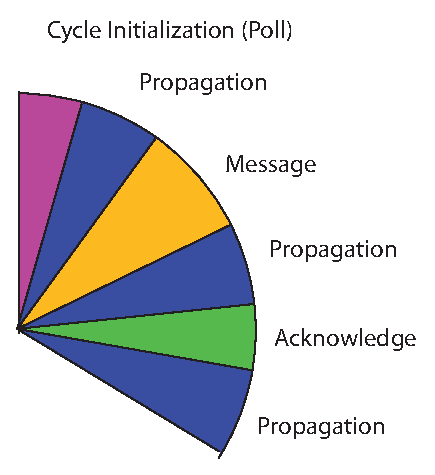
\includegraphics[width=0.2\textwidth]{slots_polled.eps}\label{fig:slots_polled}}\hfil
	\subfloat[Decentralized TDMA]{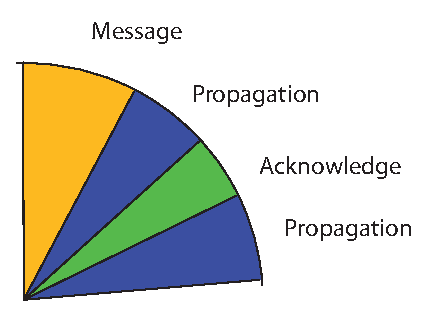
\includegraphics[width=0.2\textwidth]{slots_decentralized.eps}\label{fig:slots_decentralized}}}
\caption{Comparison of the time needed for a single slot for the two types of TDMA supported by pAcommsHandler. Eq. \ref{eq:mac_time} gives the additional length of time required by the Centralized variant.}
\label{fig:slots}
\end{figure}

\begin{figure}
\centering
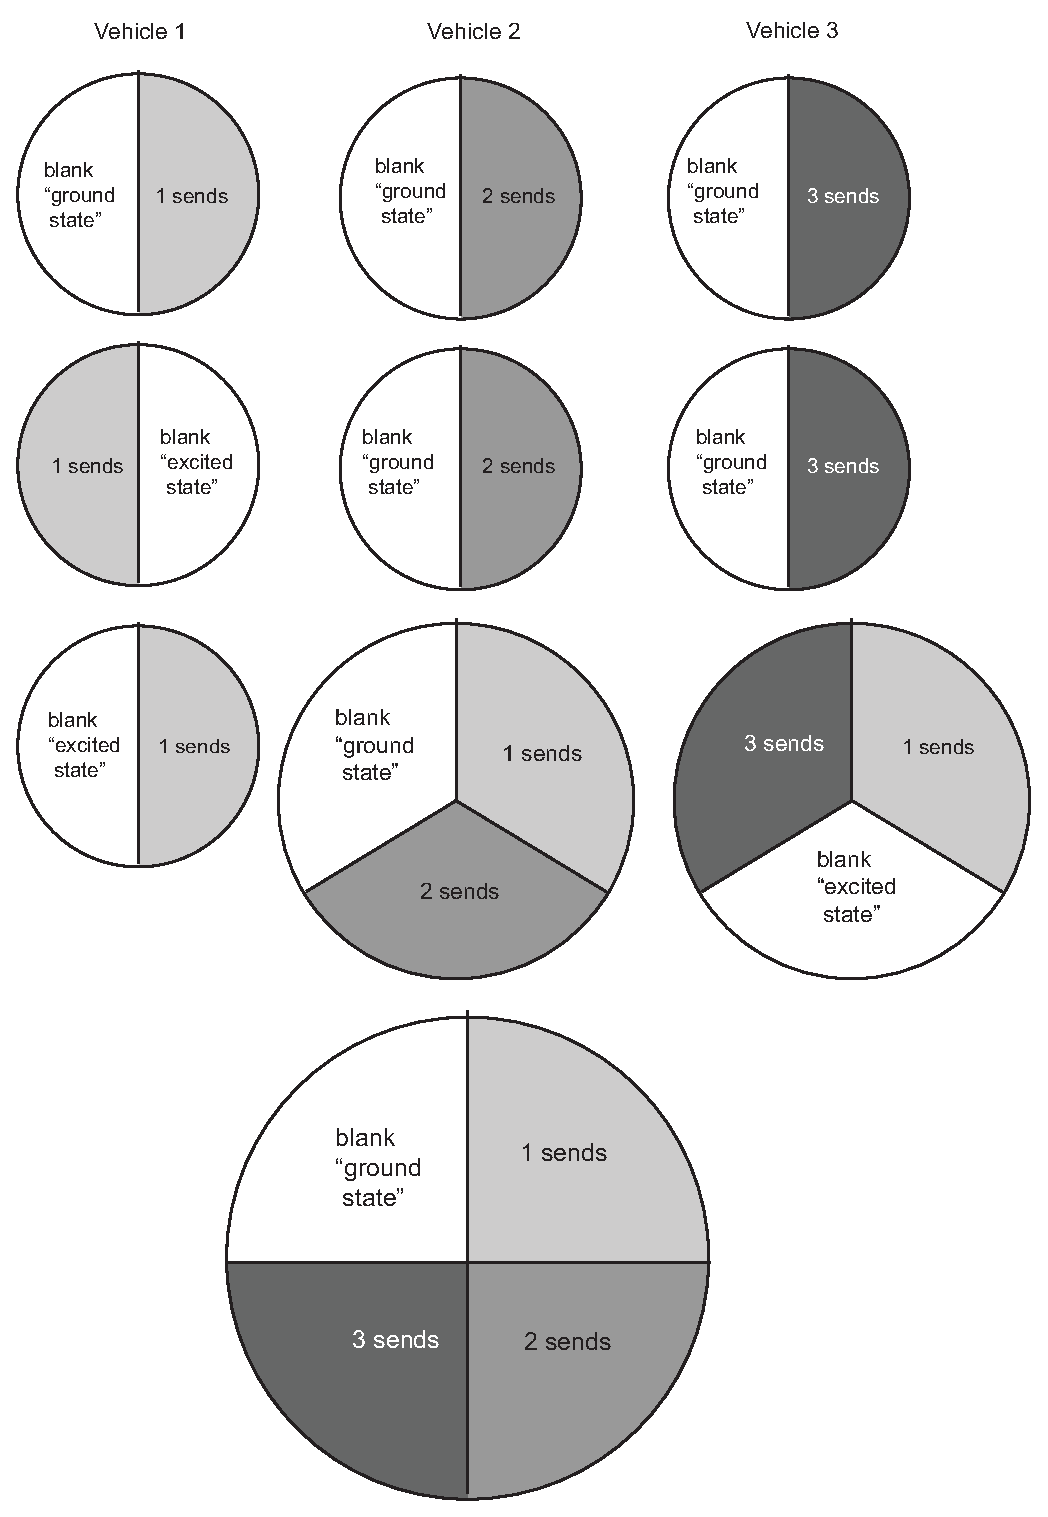
\includegraphics[width=0.5\textwidth]{slots.eps}
\caption{Graphical example of auto discovery for three nodes launched at the same time. Each circle represents the vehicle's cycle at each time step (represented by horizontal rows) based on the vehicle's current knowledge of the world. In the first row, all vehicles only know of themselves and put the blank slot in the last slot; thus, all communications collide and no discoveries are made. In the second row, vehicle 1's blank is moved (by pseudo-chance) to the penultimate (first) slot, so vehicles 2 and 3 discover 1. Then, in the third row vehicles 2 and 3 are discovered by the others because vehicle 3 moves its blank slot. By the fourth row all vehicles have discovered the others and continue to transmit without collision following the cycle diagrammed on this row.} 
\label{fig:decentralized_cycles}
\end{figure}

\subsubsection{Decentralized TDMA with passive auto-discovery}

Decentralized TDMA removes the cycle initialization packet and thus reduces the length of each slot and the chance of errors. However, it introduces the constraint of synchronized clocks\footnote{the accuracy of the clock synchronization can be  low relative to other timing needs such as bi-static sonar. Generally, accuracy better than 0.1 seconds is acceptable; higher inaccuracies can be handled by increasing the guard time on both sides of each slot.} for all nodes, which can be somewhat tricky to maintain underwater.

Decentralized TDMA gives each vehicle a single slot in which it transmits. Each vehicle initiates its own transmission at the start of its slot. Collisions are avoided by each vehicle following the same rules about slot placement within the time window (based on the time of day). All slots are ordered by ascending acoustic MAC address (or ``modem identification number''), which is an unsigned integer unique for each network.

During the runtime of the network, it is often desirable to add or remove nodes. Since the MAC is spread throughout the nodes, there is no easy way to change the cycle during runtime. \textit{libamac} supports passive auto-discovery (and subsequent expiration) of nodes to provide a solution to this problem. This auto-discovery is passive because it requires no control messaging beyond the normal communications between nodes.

Vehicles are discovered by shifting a blank slot in each cycle based on their knowledge of the world and the time of day. If a new vehicle is heard from during the blank, it is added to the listening vehicle's knowledge of the world and hence their cycle. In the simplified situation (which is really a worst case scenario) discovery is defined by a single vehicle transmitting during a cycle and all the others silent (the current slot is not equal to each vehicle's acoustic MAC address).

\begin{table}
\centering
\begin{tabular}{|c|c|c|c|}
\hline time & vehicle 1 & vehicle 2 & result \\ 
\hline 0   & send       & send  & collision \\ 
\hline 15  & blank      & blank & nothing \\ 
\hline 30  & blank      & send  & success: 1 discovers 2 \\ 
\hline 45  & cycle wait & blank & nothing \\ 
\hline 60  & cycle wait & send  & success \\ 
\hline 75  & cycle wait & blank & nothing \\ 
\hline 90  & send       & blank & success: 2 discovers 1 \\ 
\hline 105 & listen for 2 & cycle wait & nothing \\ 
\hline 120 & blank & cycle wait & nothing \\ 
\hline 135 & send & listen for 1 & success \\ 
\hline 150 & listen for 2 & send & success \\ 
\hline 165 & blank & blank & nothing \\ 
\hline 180 & send & listen for 1 & success \\ 
\hline 195 & blank & blank & nothing \\ 
\hline 210 & listen for 2 & send & success \\ 
\hline 
\end{tabular} 
\caption{Example initialization for the Decentralized TDMA with autodiscovery. By 135 seconds, both vehicles have discovered each other and are synchronized. Thus, no more collisions will occur. This scenario assumes that both vehicles always have some data to send during their slot.}
\end{table}

\subsection{Simple complete example MOOS files}

\subsubsection{Example 1: Basic CCL (goby/share/cfg/MOOS/basic\_ccl)}\label{sec:moos_example_1}
This example sends the bytes !0x020304! from node 1 (!mm1!) to node 2 (!mm2!). It shows use of all the parts of pAcommsHandler except the DCCL encoding / decoding unit. I use !iModemSim! here to simulate the WHOI Micro-Modem. This process is available in moos-ivp-local (\url{http://oceanai.mit.edu/moos-ivp/pmwiki/pmwiki.php?n=Support.Milocal}). You can also easily substitute real modems by removing iModemSim references and changing the !serial_port!.

\paragraph{MOOS file for Node 1: goby/share/cfg/MOOS/basic\_ccl/mm1.moos}
\boxedverbatiminput{"@RELATIVE_CMAKE_SOURCE_DIR@/share/cfg/MOOS/basic_ccl/mm1.moos"}
\resetbvlinenumber

\paragraph{MOOS file for Node 2: goby/share/cfg/MOOS/basic\_ccl/mm2.moos}
\boxedverbatiminput{"@RELATIVE_CMAKE_SOURCE_DIR@/share/cfg/MOOS/basic_ccl/mm2.moos"}
\resetbvlinenumber

\subsubsection{Example 2: DCCL and CCL (goby/share/cfg/MOOS/ccl\_and\_dccl)}
This example sends the DCCL ``Simple Status'' messsage from node 1 (!mm1!) to node 2 (!mm2!). !mm2! sends the REMUS CCL State message to !mm1!. It thus uses all the components of pAcommsHandler. As in the previous example, you can use real modems by removing iModemSim and changing the !serial_port! to the proper real serial port.

\paragraph{MOOS file for Node 1: goby/share/cfg/MOOS/ccl\_and\_dccl/mm1.moos}
\boxedverbatiminput{"@RELATIVE_CMAKE_SOURCE_DIR@/share/cfg/MOOS/ccl_and_dccl/mm1.moos"}
\resetbvlinenumber

\paragraph{MOOS file for Node 2: goby/share/cfg/MOOS/ccl\_and\_dccl/mm2.moos}
\boxedverbatiminput{"@RELATIVE_CMAKE_SOURCE_DIR@/share/cfg/MOOS/ccl_and_dccl/mm2.moos"}
\resetbvlinenumber

\paragraph{XML definition of Simple Status: goby/xml/simple\_status.xml}
\boxedverbatiminput{"@RELATIVE_CMAKE_SOURCE_DIR@/share/xml/simple_status.xml"}
\resetbvlinenumber

\paragraph{Modem Lookup Table: goby/share/cfg/MOOS/ccl\_and\_dccl/modemidlookup.txt}
\boxedverbatiminput{"@RELATIVE_CMAKE_SOURCE_DIR@/share/cfg/MOOS/ccl_and_dccl/modemidlookup.txt"}
\resetbvlinenumber

\section{iCommander}\label{sec:icommander} 

!iCommander! is a topside command and control (C2) tool which provides a simple
console for issuing commands through the acoustic network. By sharing
DCCL message configuration (XML) files with !pAcommsHandler! it automatically adapts to the current message set,
without any need to change code.

\subsubsection{Parameters for the iCommander Configuration Block}
\paragraph{Example .moos file}
The moos file is simple since the bulk of the configuration is stored in separate XML files (see section \ref{sec:dccl_overview} for the configuration of these files):

\boxedverbatiminput{"@RELATIVE_CMAKE_SOURCE_DIR@/src/moos/iCommander/iCommander_complete.moos"}
\resetbvlinenumber
As with pAcommsHandler, the above configuration file can be generated at any time with the command:
\begin{boxedverbatim}
iCommander --example_config
\end{boxedverbatim}
\resetbvlinenumber


\paragraph{Filling out the .moos file}

Some of the DCCL configuration (!dccl_cfg!) parameters are not used, such as the !crypto_passphrase!. 

\begin{itemize}
\item !common!: See section \ref{sec:pAcommsHandler_moos_file}.
\item !dccl_cfg.message_file!: path to an XML file containing a message set of one or messages. These are the DCCL messages. You can also load messages XML files through the Main Menu in the program.
\item !load!: path to a file of iCommander saved message(s) to load automatically on startup. You can also load messages through the Main Menu in the program.
\end{itemize}

\subsubsection{Reference Sheet}
\paragraph{Main Menu}
\begin{boxedverbatim}
 ______________________________________________________________
|            iCommander: Vehicle Command Message Sender        |
|                        2 messages loaded.                    |
|    Main Menu:                                                |
|    > Return to active message                                |
|    > Select Message                                          |
|    > Load                                                    |
|    > Save                                                    |
|    > Import Message File                                     |
|    > Exit                                                    |
|______________________________________________________________|
\end{boxedverbatim}
\resetbvlinenumber
\begin{itemize}
\item \textit{Return to active message} - only available if you have actively edited a message this session. Choose to return to the editing screen of the last message you were editing.
\item \textit{Select Message} - pick a message type to edit. All messages are read from DCCL (dynamic compact control language) XML message files.
\item \textit{Load} - load a saved message parameters file. This allows you to save values for message fields from session to session.
\item \textit{Save} - saves all open messages to a single file for later use. These files are plain text for easy use outside iCommander.
\item \textit{Import Message File} - import another DCCL XML file for use.
\item \textit{Exit} - quit cleanly.
\end{itemize}

\paragraph{Editing screen}
\begin{boxedverbatim}

    __________________________________________________
   |                                                  |
   |Editing message variable 1 of 22: MessageType     |
   |(static) you cannot change the value of this field|
   |__________________________________________________|

   ___________________________________________________
  |                                                   | 
  |Message (Type: SENSOR_PROSECUTE)                   |
  |22 entries total                                   |
  |        {Enter} for options                        |
  |        {Up/Down} for more message variables       |
  |                                                   |
  |                                 _________________ |
  |                                |                 ||
  |1. MessageType (static)         |SENSOR_PROSECUTE ||
  |                                |_________________||
  |                                 _________________ |
  |                                |                 ||
  |2. SensorCommandType (int)      |1                ||
  |                                |_________________||
  |                                 _________________ |
  |                                |                 || 
  |3. SourcePlatformId (int)       |0                ||
  |                                |_________________||
  |                                 _________________ |
  |                                |                 ||
  |4. DestinationPlatformId (int)  |3                ||
  |                                |_________________||
  |___________________________________________________|
\end{boxedverbatim}
\resetbvlinenumber

Scroll to select the box to edit. Note that you will need to scroll up or down off the screen to see all the fields at once. The information box at the top will tell you how large the field can be based on the DCCL settings. You cannot enter a value outside these ranges. Hit enter to get the editing menu.

\paragraph{Editing menu}
\begin{boxedverbatim}
        __________________________________________________________
       |                                                          |
       |                     Choose an action                     |
       |> Return to message                                       |
       |> Send                                                    |
       |> Preview                                                 |
       |> Quick switch to another open message                    |
       |> Insert special: current time                            |
       |> Insert special: local X,Y to longitude,latitude         |
       |> Insert special: community                               |
       |> Insert special: modem id                                |
       |> Clear message                                           |
       |> Main Menu                                               |
       |                                                          |
       |                                                          |
       |__________________________________________________________|
\end{boxedverbatim}
\resetbvlinenumber
\begin{itemize}
\item \textit{Return to message}
\item \textit{Send} - publish the variables for use by pAcommsHandler
\item \textit{Preview} - preview the message to be sent in exact syntactical form
\item \textit{Quick switch to another open message} - switch to another message with information (either edited this session or loaded)
\item \textit{Insert special: current time} - insert a placeholder (``\_time'') that will be replaced with the current UNIX time when message is sent (e.g. 1236053988). \textbf{Shortcut: type 't'} directly into the field and bypass this menu.
\item \textit{Insert special: local X,Y to longitude,latitude} - insert a placeholder designator to do a UTM local grid to latitude / longitude conversion. first the latitude (Y or northings) is entered (``y(lat)1:''), then you choose where to put the longitude (X or eastings) (``x(lon)1:''). after the colon enter the desired value in meters that will be converted to latitude/longitude based in the LatOrigin/LongOrigin set in the top of the MOOS file. Note that you may have more than one pair of x/y. This is the reason for the number following ``y(lat)''/``x(lon)''. ``y(lat)1'' is paired with ``x(lon)1'', ``y(lat)2'' is paired with ``x(lon)2'', etc. \textbf{Shortcut: type 'y' or 'x' respectively} directly into the fields and bypass this menu.
\item \textit{Insert special: community} - insert the name of this MOOS community.
\item \textit{Insert special: modem id} - choose a modem id from a list of names. This is based off the modem id lookup table used by pAcommsHandler.
\item Clear message
\item Main Menu
\end{itemize}

\paragraph{Acknowledgments}
If you are using pAcommsHandler with the ACK field set to 1 (true), all acoustic message acknowledgments are displayed at the top of the screen. For example, the ack of a !LAMSS_DEPLOY! message would look like this:
\begin{boxedverbatim}
 _____________________________________________
|                                             |
|Message acknowledged from queue: LAMSS_DEPLOY|
| for destination: 5                          |
| at time: 2011-Mar-03 22:38:12               |
|_____________________________________________|
\end{boxedverbatim}
\resetbvlinenumber

Similarly, expired messages (messages that exceed their \textit{ttl} without being sent) are shown as well:
\begin{boxedverbatim}
 _____________________________________________
|                                             |
|Message expired from queue: LAMSS_DEPLOY     |
| for destination: 5                          |
| at time: 2011-Mar-03 22:38:12               |
|_____________________________________________|
\end{boxedverbatim}
\resetbvlinenumber
 
\section{pREMUSCodec}

\paragraph{Example .moos file}

\boxedverbatiminput{"@RELATIVE_CMAKE_SOURCE_DIR@/src/moos/pREMUSCodec/pREMUSCodec_complete.moos"}
\resetbvlinenumber
As with pAcommsHandler, the above configuration file can be generated at any time with the command:
\begin{boxedverbatim}
pREMUSCodec --example_config
\end{boxedverbatim}

This codec handles several of the standard REMUS CCL messages. It can be configured to generate CCL State messages at regular intervals, and it will translate incoming CCL State messages into the standard !NODE_REPORT! format used internally in the LAMSS autonomy systems. This codec allows a MOOS vehicle to perform collaborative behaviors, such as collision avoidance, with a non-MOOS, standard CCL vehicle. See section \ref{sec:moos_example_1} for an example of using pREMUSCodec.

\section{iMOOS2SQL}

This is a transponder process, which translates Status, Contact, and
Track Reports into a format for interfacing the MOOS C2 with the
generic Google Earth-based (geov) topside display, e.g. as shown in
Fig.~\ref{bistatic3}. This module is available in moos-ivp-local (\url{http://oceanai.mit.edu/moos-ivp/pmwiki/pmwiki.php?n=Support.Milocal}).


\section{pGeneralCodec}

\textit{Deprecated. Do not use, rather use pAcommsHandler with no driver, no MAC, and no queueing if only encoding/decoding is desired.}

\section{pBTRCodec}

\textit{Deprecated. Do not use, rather use the \xmltag{array\_length} feature of pAcommsHandler which provides the same functionality.}

\section{pCTDCodec}

\textit{Deprecated. Do not use, rather use the \xmltag{max\_delta} feature of pAcommsHandler which provides all the same functionality but with much more generality. }

\section{pAcommsPoller}

\textit{Deprecated. Use the MAC built into pAcommsHandler. }

\DeleteShortVerb{\!}
